% !TeX program = pdflatex
% !TeX root = FCMultiLoopTID.tex

\documentclass[../FeynCalcManual.tex]{subfiles}
\begin{document}
\hypertarget{fcmultilooptid}{
\section{FCMultiLoopTID}\label{fcmultilooptid}\index{FCMultiLoopTID}}

\texttt{FCMultiLoopTID[\allowbreak{}amp,\ \allowbreak{}\{\allowbreak{}q1,\ \allowbreak{}q2,\ \allowbreak{}...\}]}
does a multi-loop tensor integral decomposition, transforming the
Lorentz indices away from the loop momenta
\texttt{q1,\ \allowbreak{}q2,\ \allowbreak{}...} The decomposition is
applied only to the loop integrals where loop momenta are contracted
with Dirac matrices or epsilon tensors.

\subsection{See also}

\hyperlink{toc}{Overview},
\hyperlink{fcloopfindtensorbasis}{FCLoopFindTensorBasis},
\hyperlink{tid}{TID}.

\subsection{Examples}

\begin{Shaded}
\begin{Highlighting}[]
\NormalTok{FCI}\OperatorTok{[}\NormalTok{FVD}\OperatorTok{[}\NormalTok{q1}\OperatorTok{,} \SpecialCharTok{\textbackslash{}}\OperatorTok{[}\NormalTok{Mu}\OperatorTok{]]}\NormalTok{ FVD}\OperatorTok{[}\NormalTok{q2}\OperatorTok{,} \SpecialCharTok{\textbackslash{}}\OperatorTok{[}\NormalTok{Nu}\OperatorTok{]]}\NormalTok{ FAD}\OperatorTok{[}\NormalTok{q1}\OperatorTok{,}\NormalTok{ q2}\OperatorTok{,} \OperatorTok{\{}\NormalTok{q1 }\SpecialCharTok{{-}}\NormalTok{ p1}\OperatorTok{\},} \OperatorTok{\{}\NormalTok{q2 }\SpecialCharTok{{-}}\NormalTok{ p1}\OperatorTok{\},} \OperatorTok{\{}\NormalTok{q1 }\SpecialCharTok{{-}}\NormalTok{ q2}\OperatorTok{\}]]} 
 
\NormalTok{FCMultiLoopTID}\OperatorTok{[}\SpecialCharTok{\%}\OperatorTok{,} \OperatorTok{\{}\NormalTok{q1}\OperatorTok{,}\NormalTok{ q2}\OperatorTok{\}]}
\end{Highlighting}
\end{Shaded}

\begin{dmath*}\breakingcomma
\frac{\text{q1}^{\mu } \;\text{q2}^{\nu }}{\text{q1}^2.\text{q2}^2.(\text{q1}-\text{p1})^2.(\text{q2}-\text{p1})^2.(\text{q1}-\text{q2})^2}
\end{dmath*}

\begin{dmath*}\breakingcomma
\frac{\text{p1}^{\mu } \;\text{p1}^{\nu }-\text{p1}^2 g^{\mu \nu }}{(1-D) \;\text{p1}^2 \;\text{q1}^2.\text{q2}^2.(\text{q1}-\text{p1})^2.(\text{q1}-\text{q2})^2}-\frac{\text{p1}^{\mu } \;\text{p1}^{\nu }-\text{p1}^2 g^{\mu \nu }}{2 (1-D) \;\text{p1}^2 \;\text{q1}^2.\text{q2}^2.(\text{q1}-\text{p1})^2.(\text{q2}-\text{p1})^2}-\frac{D \;\text{p1}^{\mu } \;\text{p1}^{\nu }-\text{p1}^2 g^{\mu \nu }}{4 (1-D) \;\text{q1}^2.\text{q2}^2.(\text{q1}-\text{p1})^2.(\text{q1}-\text{q2})^2.(\text{q2}-\text{p1})^2}+\frac{D \;\text{p1}^{\mu } \;\text{p1}^{\nu }-\text{p1}^2 g^{\mu \nu }}{2 (1-D) \;\text{p1}^4 \;\text{q1}^2.(\text{q1}-\text{q2})^2.(\text{q2}-\text{p1})^2}
\end{dmath*}

In the case of vanishing Gram determinants one can apply the same
procedure as in the case of TID or FCLoopTensorReduce: one uses
\texttt{FCLoopFindTensorBasis} to find a linear independent basis of
external momenta and then supplies this basis to the function.

\begin{Shaded}
\begin{Highlighting}[]
\NormalTok{FCClearScalarProducts}\OperatorTok{[]}
\NormalTok{SPD}\OperatorTok{[}\NormalTok{p1}\OperatorTok{]} \ExtensionTok{=}\NormalTok{ m1}\SpecialCharTok{\^{}}\DecValTok{2}\NormalTok{;}
\NormalTok{SPD}\OperatorTok{[}\NormalTok{p2}\OperatorTok{]} \ExtensionTok{=}\NormalTok{ m2}\SpecialCharTok{\^{}}\DecValTok{2}\NormalTok{;}
\NormalTok{SPD}\OperatorTok{[}\NormalTok{p1}\OperatorTok{,}\NormalTok{ p2}\OperatorTok{]} \ExtensionTok{=}\NormalTok{ m1 m2;}
\end{Highlighting}
\end{Shaded}

\begin{Shaded}
\begin{Highlighting}[]
\NormalTok{FCMultiLoopTID}\OperatorTok{[}\NormalTok{FVD}\OperatorTok{[}\NormalTok{q1}\OperatorTok{,}\NormalTok{ mu}\OperatorTok{]}\NormalTok{ FAD}\OperatorTok{[\{}\NormalTok{q1}\OperatorTok{,} \FunctionTok{m}\OperatorTok{\},} \OperatorTok{\{}\NormalTok{q1 }\SpecialCharTok{+}\NormalTok{ p1}\OperatorTok{\},} \OperatorTok{\{}\NormalTok{q1 }\SpecialCharTok{+}\NormalTok{ p2}\OperatorTok{\}],} \OperatorTok{\{}\NormalTok{q1}\OperatorTok{\}]}
\end{Highlighting}
\end{Shaded}

\FloatBarrier
\begin{figure}[!ht]
\centering
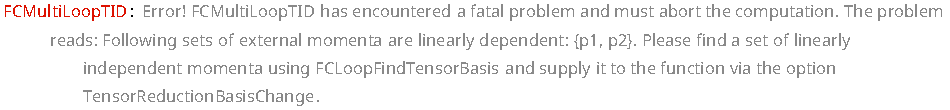
\includegraphics[width=0.6\linewidth]{img/0h2gltw65l2pe.pdf}
\end{figure}
\FloatBarrier

\begin{dmath*}\breakingcomma
\text{\$Aborted}
\end{dmath*}

\begin{Shaded}
\begin{Highlighting}[]
\NormalTok{FCLoopFindTensorBasis}\OperatorTok{[\{}\NormalTok{p1}\OperatorTok{,}\NormalTok{ p2}\OperatorTok{\},} \OperatorTok{\{\},} \FunctionTok{n}\OperatorTok{]}
\end{Highlighting}
\end{Shaded}

\begin{dmath*}\breakingcomma
\left(
\begin{array}{c}
 \;\text{p1} \\
 \;\text{p2} \\
 \;\text{p2}\to \;\text{p1} \;\text{FCGV}(\text{Prefactor})\left(\frac{\text{m2}}{\text{m1}}\right) \\
\end{array}
\right)
\end{dmath*}

\begin{Shaded}
\begin{Highlighting}[]
\NormalTok{FCMultiLoopTID}\OperatorTok{[}\NormalTok{FVD}\OperatorTok{[}\NormalTok{q1}\OperatorTok{,}\NormalTok{ mu}\OperatorTok{]}\NormalTok{ FAD}\OperatorTok{[\{}\NormalTok{q1}\OperatorTok{,} \FunctionTok{m}\OperatorTok{\},} \OperatorTok{\{}\NormalTok{q1 }\SpecialCharTok{+}\NormalTok{ p1}\OperatorTok{\},} \OperatorTok{\{}\NormalTok{q1 }\SpecialCharTok{+}\NormalTok{ p2}\OperatorTok{\}],} \OperatorTok{\{}\NormalTok{q1}\OperatorTok{\},} 
\NormalTok{  TensorReductionBasisChange }\OtherTok{{-}\textgreater{}} \OperatorTok{\{\{}\NormalTok{p1}\OperatorTok{,}\NormalTok{ p2}\OperatorTok{\}} \OtherTok{{-}\textgreater{}} \OperatorTok{\{}\NormalTok{p1}\OperatorTok{\}\}]}
\end{Highlighting}
\end{Shaded}

\begin{dmath*}\breakingcomma
\frac{\text{p1}^{\text{mu}}}{2 \;\text{m1}^2 \;\text{q1}^2.\left((\text{q1}-\text{p2})^2-m^2\right)}-\frac{\left(m^2+\text{m1}^2\right) \;\text{p1}^{\text{mu}}}{2 \;\text{m1}^2 \left(\text{q1}^2-m^2\right).(\text{q1}-\text{p1})^2.(\text{q1}-\text{p2})^2}-\frac{\text{p1}^{\text{mu}}}{2 \;\text{m1}^2 \;\text{q1}^2.(-\text{p1}+\text{p2}+\text{q1})^2}
\end{dmath*}
\end{document}
